%% 
%% Copyright 2019-2024 Elsevier Ltd
%% 
%% This file is part of the 'CAS Bundle'.
%% --------------------------------------
%% 
%% It may be distributed under the conditions of the LaTeX Project Public
%% License, either version 1.3c of this license or (at your option) any
%% later version.  The latest version of this license is in
%%    http://www.latex-project.org/lppl.txt
%% and version 1.3c or later is part of all distributions of LaTeX
%% version 1999/12/01 or later.
%% 
%% The list of all files belonging to the 'CAS Bundle' is
%% given in the file `manifest.txt'.
%% 
%% Template article for cas-dc documentclass for 
%% double column output.

\documentclass[pdflatex]{cas-dc}

% Packages used by the manuscript
\usepackage{natbib}
\usepackage{amsthm}
\usepackage{booktabs}
\usepackage{tabularx}
\usepackage{xcolor}
\usepackage{enumitem}
\usepackage{float}
\usepackage{placeins}
\usepackage{algorithm}
\usepackage{algpseudocode}
\usepackage{tikz}
\usetikzlibrary{svg.path}
\usepackage{graphicx}
\usepackage{orcidlink}

\hypersetup{
  colorlinks = true,
  linkcolor  = blue,
  citecolor  = blue,
  urlcolor   = blue
}

\theoremstyle{remark}
\newtheorem{remark}{Remark}
\theoremstyle{plain}
\newtheorem{theorem}{Theorem}
\newtheorem{corollary}[theorem]{Corollary}

\setcounter{topnumber}{5}
\setcounter{bottomnumber}{5}
\setcounter{totalnumber}{10}
\renewcommand{\topfraction}{0.95}
\renewcommand{\bottomfraction}{0.95}
\renewcommand{\textfraction}{0.05}
\renewcommand{\floatpagefraction}{0.90}

\begin{document}
\let\WriteBookmarks\relax
\def\floatpagepagefraction{1}
\def\textpagefraction{.001}
% Add these two lines:

% Short title
\shorttitle{Frozen UNI for Breast Cancer Phenotyping}    

% Short author
% \shortauthors{}  

% Main title of the paper
\title [mode = title]{Cross Site Evaluation and Calibration of Frozen UNI Representations for Breast Cancer Molecular Phenotype Prediction}  

% Title footnote mark
% eg: \tnotemark[1]
\tnotemark[1] 

% Title footnote 1.
% eg: \tnotetext[1]{Title footnote text}
\tnotetext[1]{} 

% First author
%
% Options: Use if required
% eg: \author[1,3]{Author Name}[type=editor,
%       style=chinese,
%       auid=000,
%       bioid=1,
%       prefix=Sir,
%       orcid=0000-0000-0000-0000,
%       facebook=<facebook id>,
%       twitter=<twitter id>,
%       linkedin=<linkedin id>,
%       gplus=<gplus id>]

\author[1,3]{Chigozie Athanasius Nnadiekwe} 
[orcid=0009-0000-6014-2703]
\credit{Conceptualization, Methodology, Software, Formal analysis,
Investigation, Validation, Data curation, Visualization,
Writing original draft, Writing review \& editing}

\author[2]{Simeon Okechukwu Ajakwe}
    [orcid=0000-0002-6973-530X]
\credit{Supervision, Formal analysis, Validation, Investigation,
Writing review \& editing}

\author[1]{Goodness Ebube Okwuosa}
[orcid=0009-0002-1230-4354]
\credit{Methodology, Software, Validation, Investigation, Data curation}

\author[1]{Jae Min Lee}
 [orcid=0000-0001-6885-5185]
\credit{Project administration, Validation, Resources, Writing review \& editing}

\author[1]{Dong-Seong Kim}[
  orcid=0000-0002-2977-5964]
\cormark[1]
\ead{dskim@kumoh.ac.kr}
% \ead[url]{https://orcid.org/0000-0002-2977-5964}
\credit{Supervision, Project administration, Funding acquisition, Resources,
Writing review \& editing}

\affiliation[1]{organization={Department of IT Convergence Engineering},
            addressline={Kumoh National Institute of Technology},
            city={Gumi},
            postcode={39177},
            country={Republic of Korea}}

\affiliation[2]{organization={Smart Computing Department},
            addressline={Kyungdong University, Global Campus},
            city={Goseong-gun, Gangwon Province},
            postcode={24764},
            country={Republic of Korea}}

\affiliation[3]{organization={Department of Biomedical Engineering},
            addressline={David Umahi Federal University of Health Sciences},
            city={Uburu, Ebonyi State},
            postcode={491105},
            country={Nigeria}}

\cortext[1]{Corresponding author}
% Footnote text
\fntext[1]{}

% For a title note without a number/mark
%\nonumnote{}

% Here goes the abstract

\begin{abstract}
\noindent\textbf{Background:}
Histology-based molecular prediction may support breast-cancer assessment, but reliable probabilities and cross-site performance remain uncertain. We evaluated frozen UNI representations across five molecular endpoints.
\noindent\textbf{Methods:}
Diagnostic whole-slide images from 345 TCGA-BRCA patients yielded 345,937 quality-controlled patches from 347 slides. Hierarchical mean pooling generated patient representations for logistic-regression prediction of estrogen receptor (ER), progesterone receptor (PR), HER2, \textit{PIK3CA} mutation, and four-class PAM50. Evaluation used patient-separated five-fold cross-validation and four within-TCGA site holdouts, with development-only model fitting and calibration.
\noindent\textbf{Results:}
Pooled calibrated AUROCs were 0.843 for ER, 0.768 for PR, 0.672 for HER2, and 0.589 for \textit{PIK3CA}; raw PAM50 macro-AUROC was 0.858. Mean calibrated site-held-out AUROCs were 0.869, 0.781, 0.656, 0.613, and 0.809, respectively. Binary Brier scores decreased by 0.019--0.089, with calibration slopes approaching one, whereas PAM50 showed no clear calibration benefit. HER2 performance varied most across sites. L2 normalisation produced a nominal improvement in \textit{PIK3CA} discrimination, while principal-component compression reduced PAM50 macro-AUROC.
\noindent\textbf{Conclusions:}
Frozen UNI representations showed endpoint-dependent discrimination and probability reliability. The findings support further investigation of adjunctive molecular-testing applications, but do not establish assay replacement or independent external validity.

\end{abstract}
\begin{keywords}
Breast cancer \sep
Computational pathology \sep
Whole-slide imaging \sep
Molecular phenotype prediction \sep
Pathology foundation models \sep
Probability calibration \sep
Cross-site evaluation
\end{keywords}
\maketitle
\section{Introduction}\label{sec:introduction}
% Numbered list
% Use the style of numbering in square brackets.
% If nothing is used, default style will be taken.
%\begin{enumerate}[a)]
%\item 
%\item 
%\item 
%\end{enumerate}  

Breast cancer classification and treatment rely on molecular characterization. Estrogen receptor (ER), progesterone receptor (PR), and human epidermal growth factor receptor 2 (HER2) status inform systemic treatment, while PAM50 identifies intrinsic subtypes with prognostic relevance \citep{TCGA2012,Parker2009}. \textit{PIK3CA} mutation status can determine eligibility for targeted therapy \citep{Andre2019}. These biomarkers require immunohistochemical, molecular, or gene-expression assays. Routine haematoxylin-and-eosin (H\&E) histology also contains morphological signals associated with these phenotypes, raising the possibility of supporting confirmatory-testing prioritisation.

Computational pathology models extract predictive information from whole-slide images (WSIs) without exhaustive annotation \citep{Campanella2019,Lu2021}. Studies have linked histology to genomic alterations and transcriptomic programmes \citep{Kather2020,Fu2020,Schmauch2020}, and breast-cancer studies have investigated receptor status, intrinsic subtype, mutations, gene expression, treatment response, heterogeneity, and survival \citep{Couture2018,Rawat2020,Wang2021BRCA,Qu2021,Ektefaie2021,Duanmu2022,Liu2024Protein,Wang2023ITH,Ekholm2024,Frascarelli2024}. Some include independent cohorts \citep{Liu2024Protein,Ekholm2024,Miao2026}, but differences in endpoints, cohorts, and validation designs preclude direct performance comparisons (Table~\ref{tab:sota}). These findings support morphology-linked molecular prediction, without establishing equivalence to definitive assays.

Pathology foundation models, including UNI, provide reusable representations for downstream prediction \citep{Chen2024UNI,Vorontsov2024,Ding2025}. Freezing the encoder permits relatively simple models in moderate-sized cohorts, but does not ensure reliable probabilities or transportability. Staining, scanning, tissue processing, and case-mix differences can impair performance \citep{Zech2018,Tellez2019,Howard2021,Jahanifar2025}. Random patient splits may distribute institution-associated signatures across development and evaluation sets, obscuring site-specific weaknesses \citep{Howard2021}. Moreover, discrimination measures patient ranking, whereas calibration measures agreement between predicted probabilities and observed outcomes \citep{VanCalster2019}. Strong discrimination can coexist with miscalibration \citep{Guo2017,Minderer2021}; both therefore require evaluation.

We evaluated frozen UNI representations for ER, PR, HER2, \textit{PIK3CA}, and four-class PAM50 in TCGA-BRCA. Image-quality criteria, labels, and patient partitions were fixed before evaluation. Hierarchical pooling generated patient representations for five-fold cross-validation and four within-TCGA site holdouts. We assessed discrimination, probability calibration, and the effects of L2 normalisation and principal-component compression. The objective was to determine which molecular phenotypes were captured by frozen representations and whether their predictions remained reliable across source sites. The site holdouts assess within-TCGA transportability rather than independent external validity.

\begin{table*}[htbp]
\centering
\caption{Selected studies of breast-cancer molecular prediction from whole-slide images. Differences in targets, cohorts, and validation designs prevent direct performance comparisons. External evaluation denotes a distinct non-TCGA cohort. NR, not reported.}
\label{tab:sota}
\footnotesize
\renewcommand{\arraystretch}{1.10}
\setlength{\tabcolsep}{3pt}

\begin{tabularx}{\textwidth}{
@{}
>{\raggedright\arraybackslash}p{1.55cm}
>{\raggedright\arraybackslash}p{2.05cm}
>{\raggedright\arraybackslash}p{2.35cm}
>{\raggedright\arraybackslash}X
>{\raggedright\arraybackslash}p{2.30cm}
@{}}
\toprule
\textbf{Study} &
\textbf{Targets} &
\textbf{Representation} &
\textbf{Validation} &
\textbf{Calibration} \\
\midrule

Couture et al.~\citep{Couture2018}
& Grade, ER, histology, intrinsic subtype
& Patch CNN; slide aggregation
& Internal TCGA-BRCA
& NR \\

Rawat et al.~\citep{Rawat2020}
& ER, PR, HER2
& Deep tissue representations
& Internal TCGA-BRCA
& NR \\

Wang et al.~\citep{Wang2021BRCA}
& Germline \textit{BRCA1}/\textit{BRCA2} mutation
& Multiscale residual network
& TCGA development; 64-case external cohort
& NR \\

Qu et al.~\citep{Qu2021}
& Somatic mutations, pathways
& Self-attention tile weighting
& TCGA-BRCA; cross-cancer transfer
& NR \\

Ektefaie et al.~\citep{Ektefaie2021}
& Receptor status, breast-cancer classes
& Histology--multi-omics integration
& TCGA-BRCA; selected tasks in two independent cohorts
& NR \\

Duanmu et al.~\citep{Duanmu2022}
& Pathological complete response
& Spatial-attention network
& Retrospective internal evaluation
& NR \\

Liu et al.~\citep{Liu2024Protein}
& Protein abundance, drug response
& Contrastive features; attention pooling
& TCGA-BRCA; external CPTAC-BRCA
& NR \\

Ekholm et al.~\citep{Ekholm2024}
& Expression-based proliferation scores
& CNN-based regression
& Internal test set; 997-case external cohort
& NR \\

Miao et al.~\citep{Miao2026}
& \textit{PIK3CA} mutation
& Foundation-model features; MIL; clinical-data fusion
& TCGA development; 166 external patients from three centres
& NR \\

Present study
& ER, PR, HER2, \textit{PIK3CA}, four-class PAM50
& Frozen UNI; hierarchical mean pooling
& Patient-separated five-fold cross-validation; four within-TCGA site holdouts
& Internal: sigmoid; holdouts: sigmoid for binary endpoints, temperature scaling for PAM50 \\

\bottomrule
\end{tabularx}
\end{table*}

Table~\ref{tab:sota} summarises selected breast-cancer WSI studies, highlighting differences in prediction targets, representations, validation designs, and reported calibration.



\section{Materials and methods}

\subsection{Study population and endpoints}

This retrospective study used de-identified diagnostic H\&E WSIs and patient-level annotations from The Cancer Genome Atlas Breast Invasive Carcinoma (TCGA-BRCA) project \citep{TCGA2012}. The patient was the modelling and evaluation unit (Fig.~\ref{fig:design}). Under the authors' institutional policy, additional ethics approval and consent were not required. Sample size depended on imaging, label, acquisition, and quality-control criteria; no prospective calculation was performed.

A Genomic Data Commons (GDC) audit on 14 September 2026 identified 1,133 diagnostic-slide files from 1,062 patients; restriction to primary-tumour samples yielded 1,132 WSIs from 1,061 patients. The study combined an initial acquisition of 91 patients and 93 WSIs with 254 non-overlapping patients, each contributing one WSI from Tissue Source Site (TSS) codes A2 (11), C8 (46), E2 (71), and BH (126), yielding 345 patients and 347 WSIs. Non-acquired cases were outside the sampling design, not quality-control failures. Slide barcodes were matched to patient identifiers and acquisition manifests; neither patients nor slides overlapped between stages. TSS codes served as source-domain proxies. Holdout sites were selected before performance evaluation using the feasibility of endpoint and class counts, and included all eligible acquired patients from each TSS irrespective of acquisition stage.

ER, PR, and HER2 labels came from the locked clinical source. ER and PR required definitive positive or negative assessments; equivocal, indeterminate, or missing HER2 assessments were excluded. PanCancer Atlas PAM50 labels defined four classes: luminal A, luminal B, basal-like, and HER2-enriched. Normal-like cases and missing subtype labels were excluded. Within a verified mutation-profiled denominator, \textit{PIK3CA}-positive cases had qualifying missense mutations or in-frame deletions; wild-type cases were profiled patients without qualifying alterations. Unprofiled patients were not classified as wild type.

\begin{figure*}[htbp]
\centering
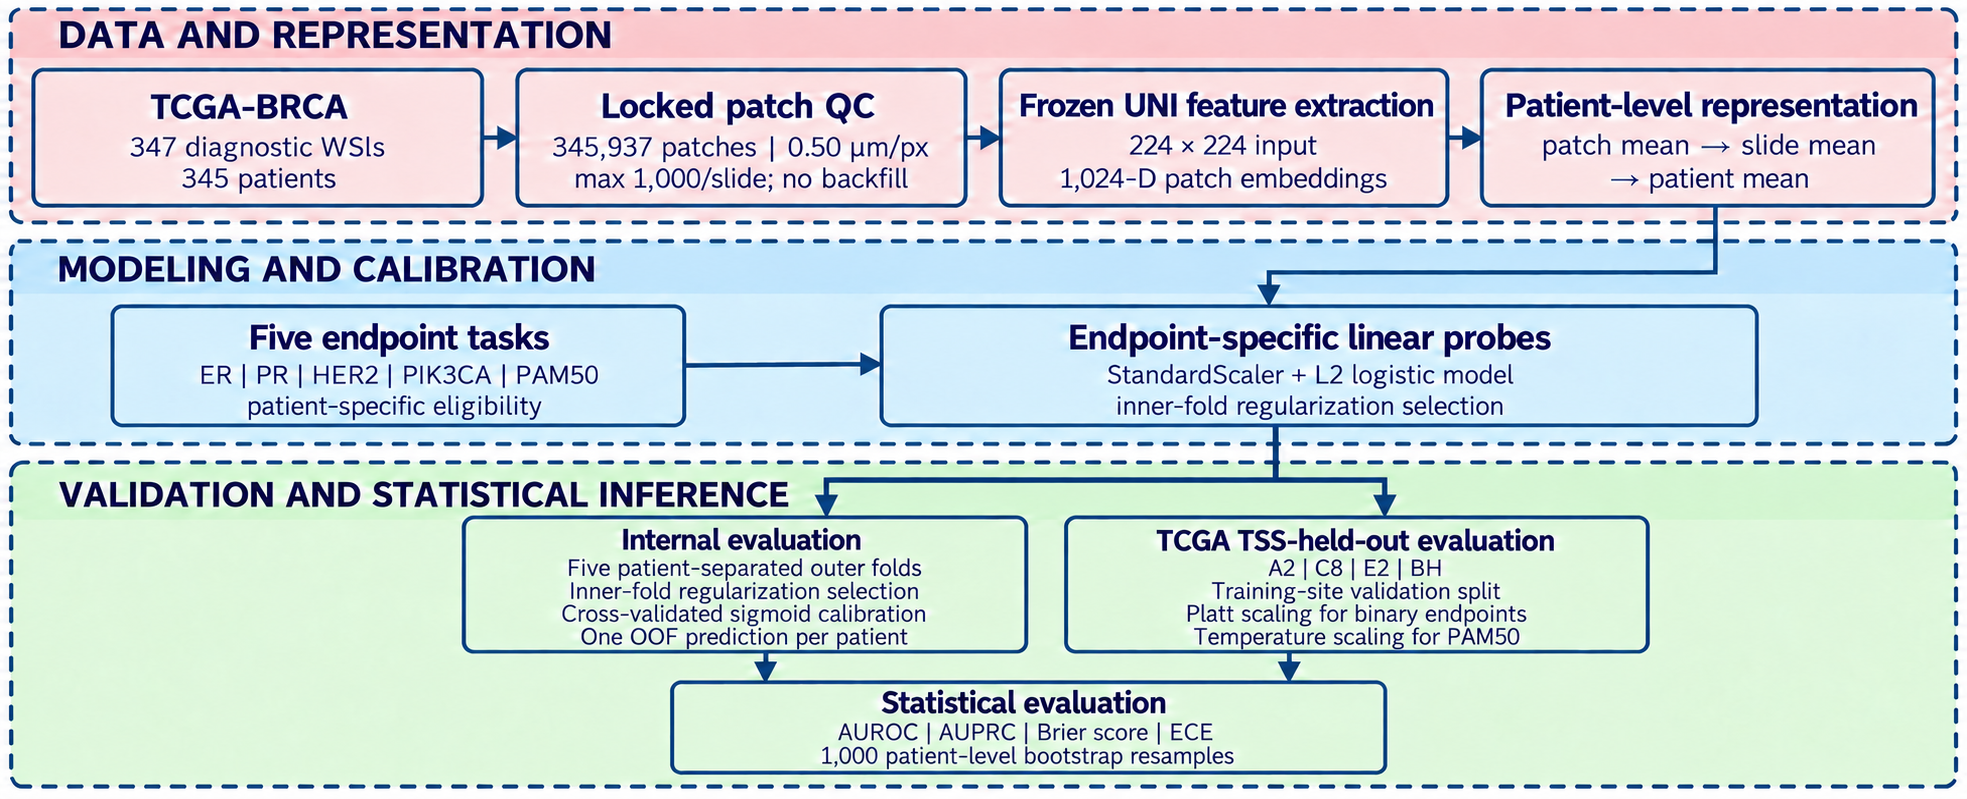
\includegraphics[width=\textwidth]{figures/Figure 1.png}
\caption{Study design and leakage-control framework. Quality-controlled patches underwent frozen UNI feature extraction and hierarchical patch-to-slide-to-patient aggregation. Patient representations were evaluated using five-fold out-of-fold prediction and four within-TCGA site holdouts. Preprocessing, model selection, and calibration used development data only. Site holdouts do not constitute independent external validation.}
\label{fig:design}
\end{figure*}


\subsection{Image processing and patient representations}

Patches were sampled at $0.50\,\mu\mathrm{m}$/pixel and resampled to $256\times256$ pixels. Frozen initial gates required low- and high-resolution tissue fractions of at least 0.50 and 0.35, respectively. Maximum permitted fractions were 0.05 for low-resolution green artefacts, 0.60 for white background, and 0.01 for combined green/cyan artefacts. Final retention required the average of mean green and blue intensities divided by mean red intensity (floored at $10^{-6}$) to be below 1.10, and mean local greyscale standard deviation to be at least 0.50 in $9\times9$ neighbourhoods.

Up to 1,000 initially accepted patches per WSI were selected using deterministic slide-specific sampling (seed 2026). Final rejections were not replaced. Focus was audited without exclusion; no tumour annotations or task-specific regions were used. The acquisitions retained 92,773 and 253,164 patches, respectively (345,937 total).

OpenSlide-extracted RGB patches were resized to $224\times224$ pixels and ImageNet-normalised. Frozen UNI, operated in evaluation mode, produced 1,024-dimensional embeddings without fine-tuning or stain normalisation \citep{Chen2024UNI}. Patch embeddings were averaged within slides, then slide vectors within patients. This gave one 1,024-dimensional vector per patient without weighting patients by slide or patch counts.

\subsection{Internal prediction and calibration}

Endpoint-specific, class-stratified five-fold cross-validation used seed 20260905, keeping each patient's data within one fold. Outer-training data alone fitted standardisation and class-balanced L2-regularised logistic regression; PAM50 used multinomial logistic regression. Stratified inner cross-validation selected $C$ from $\{0.001,0.01,0.1,1,10,100\}$ using average precision for binary endpoints and negative log loss for PAM50. Up to four inner folds were used, reduced when necessary for minority-class counts. The \texttt{lbfgs} solver allowed 5,000 iterations.

Internal sigmoid calibration used \texttt{CalibratedClassifierCV} with \texttt{ensemble="auto"} in scikit-learn 1.8.0, resolving to an ensemble for the cloned tuned predictive pipeline. Each inner-training fold fitted a model; its inner-validation fold fitted the calibrator. Outer-test probabilities were averaged across estimator--calibrator pairs. PAM50 used class-specific sigmoid mappings, normalised across classes before averaging. Raw predictions came from the tuned model fitted on the complete outer-training set. Each patient received raw and calibrated out-of-fold predictions. Ensemble calibration and pooling across independently fitted outer folds could change rankings relative to raw predictions.

\subsection{Site holdouts and representation comparisons}

For each endpoint, all eligible patients from one designated TSS formed the test set. Remaining-site patients supplied development data, with approximately 20\% allocated deterministically to validation within TSS-by-class strata, retaining at least one training patient in strata containing two or more. Standardisation, model selection, and fitting used training data alone. Validation data fitted sigmoid calibration on binary probability logits or PAM50 temperature scaling; temperature minimised log loss over 401 logarithmically spaced values from 0.1 to 10. Test outcomes informed none of these steps. The 20 endpoint--site experiments assessed within-TCGA transportability.

Representation comparisons used the original features, sample-wise L2 normalisation, or principal-component analysis (PCA) with 32, 64, or 128 components. L2 normalisation preceded logistic regression; PCA followed training-fitted standardisation. Model selection and all fitted transformations remained within training folds. Comparisons used paired raw pooled out-of-fold predictions (Table~\ref{tab:ablation}; Fig.~\ref{fig:ablation}).

\begin{table}[htbp]
\centering
\caption{Representation comparisons using pooled patient-level raw out-of-fold AUROC. Values are not means of fold-specific AUROCs. PAM50 values are macro-averaged one-versus-rest estimates. Fitted transformations used the corresponding outer-training folds only.}
\label{tab:ablation}
\small
\setlength{\tabcolsep}{3pt}
\renewcommand{\arraystretch}{1.15}

\begin{tabularx}{\linewidth}{
@{}l
*{5}{>{\centering\arraybackslash}X}
@{}}
\toprule
\textbf{Endpoint}
& \shortstack{\textbf{Full}\\\textbf{1,024-D}}
& \shortstack{\textbf{L2}\\\textbf{L2 norm.}}
& \textbf{PCA-32}
& \textbf{PCA-64}
& \textbf{PCA-128} \\
\midrule
ER              & 0.818 & 0.857 & 0.841 & 0.850 & 0.801 \\
PR              & 0.752 & 0.777 & 0.789 & 0.754 & 0.739 \\
HER2            & 0.647 & 0.684 & 0.682 & 0.676 & 0.664 \\
\textit{PIK3CA} & 0.555 & 0.588 & 0.609 & 0.588 & 0.592 \\
PAM50           & 0.858 & 0.856 & 0.836 & 0.840 & 0.842 \\
\bottomrule
\end{tabularx}
\end{table}

\begin{figure*}[htbp]
\centering
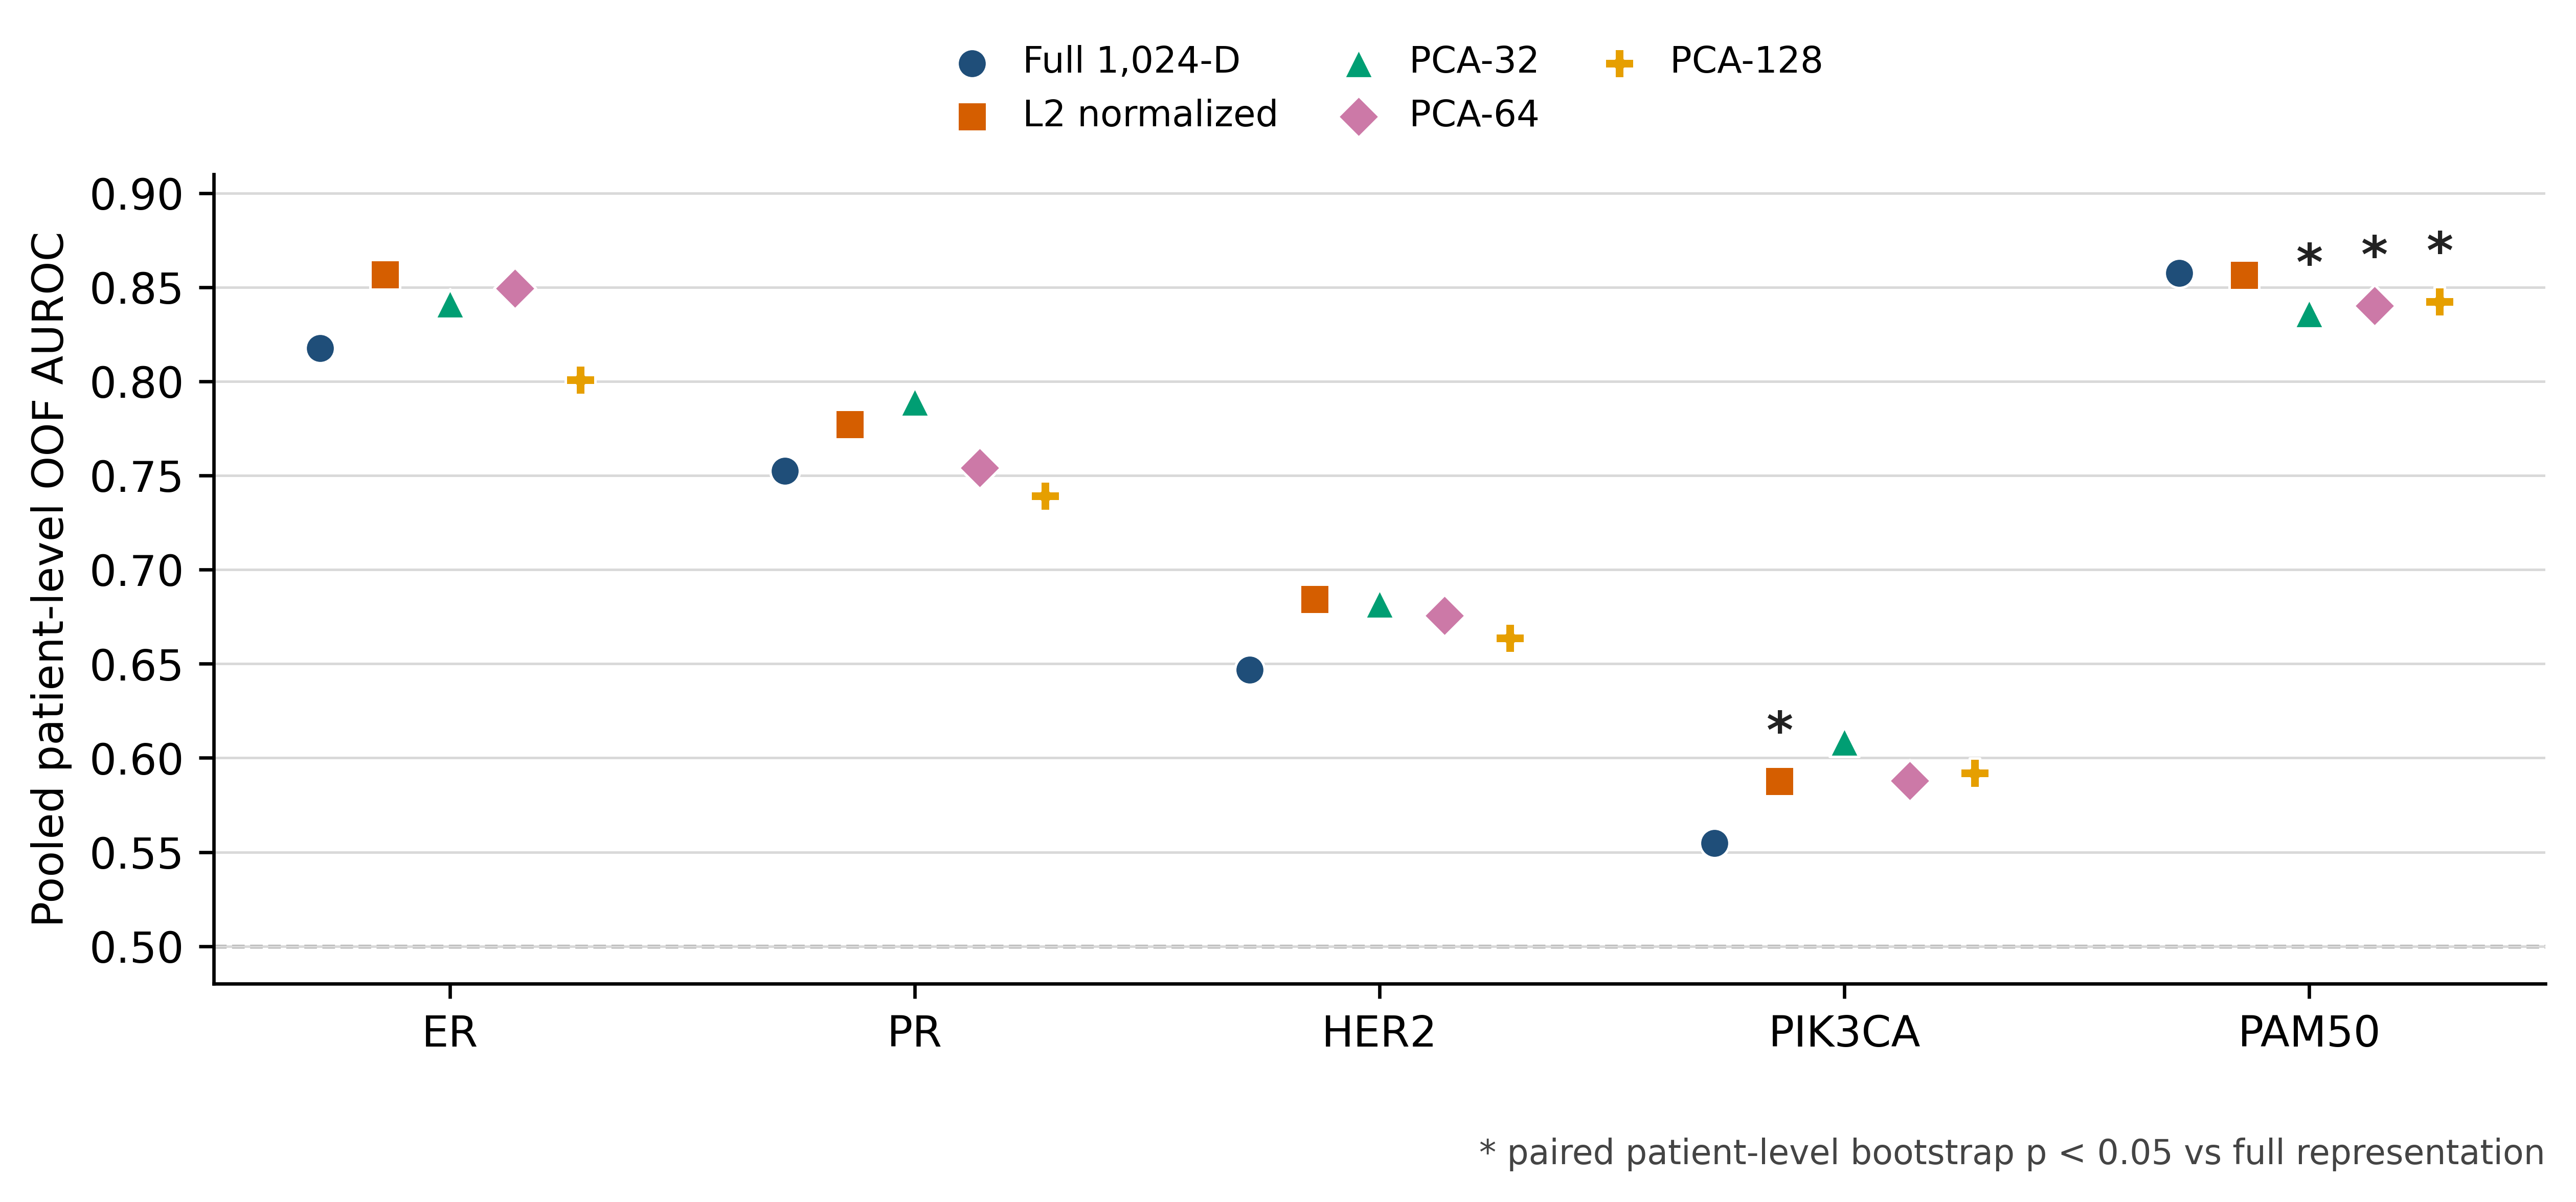
\includegraphics[width=\textwidth]{figures/Figure5_representation_ablation_pooled_oof.png}
\caption{Representation-ablation effects on pooled raw out-of-fold AUROC. Asterisks indicate nominal, unadjusted paired patient-level bootstrap $p<0.05$ relative to the full representation. PAM50 values are macro-averaged one-versus-rest AUROCs.}
\label{fig:ablation}
\end{figure*}

\subsection{Statistical analysis and reproducibility}

Discrimination measures were the areas under the receiver operating characteristic (AUROC) and precision--recall (AUPRC) curves, macro-averaged one-versus-rest for PAM50. AUPRC was interpreted against outcome prevalence. Probability accuracy used binary or unnormalised multiclass Brier scores, log loss, and top-label expected calibration error (ECE) with ten equal-width confidence bins. Balanced accuracy, macro-F1, Matthews correlation coefficient, sensitivity, and specificity used a threshold of 0.5 for binary endpoints and the highest-probability class for PAM50.

For binary endpoints and each PAM50 class, calibration-in-the-large intercepts used logistic models with predicted logits as offsets; slopes used logistic recalibration with freely estimated intercepts. Ideal values were zero and one, respectively. Probabilities were clipped to $[10^{-6},1-10^{-6}]$. Reliability diagrams used ten approximately equal-frequency bins and Wilson 95\% intervals, distinct from ECE binning; PAM50 was analysed classwise.

Internal estimates used pooled patient-level out-of-fold predictions. Percentile 95\% intervals and paired contrasts used 1,000 patient-level bootstrap replicates; undefined metrics were omitted from invalid replicates. Two-sided bootstrap $p$ values were twice the smaller sign-tail proportion, adding one to its numerator and denominator and capping the result at one. Comparisons were exploratory at nominal $p<0.05$, without multiplicity adjustment. Bootstrapping conditioned on fitted predictions rather than model retraining; pooled calibration described aggregate out-of-fold performance, not one deployable calibrator.

Site performance used unweighted means, ranges, and worst-site estimates without pooling predictions. Site-specific intervals used 1,000 within-test-group patient bootstraps (Supplementary Table~S1). The source-population audit appears in Supplementary Fig.~S1; calibration diagnostics and paired effects appear in Supplementary Tables~S2--S3 and Supplementary Fig.~S2.

Analyses used Python 3.11.9, NumPy 2.4.4, pandas 3.0.2, and scikit-learn 1.8.0; extraction additionally used PyTorch, \texttt{timm}, Pillow, and OpenSlide. Complete dependencies were archived. SHA-256 hashes and automated checks verified manifests, patient separation, counts, uniqueness, finite values, and prediction completeness. Seed 20260905 also governed bootstrap calibration analyses. Additional audits and calibration analyses used frozen outputs without retraining or changing partitions.



\section{Results}

\subsection{Cohort and internal discrimination}

The cohort comprised 345 patients, 347 WSIs, and 345,937 retained patches. Endpoint-specific sample sizes and class distributions are reported in Table~\ref{tab:cohort}; the workflow is shown in Fig.~\ref{fig:design}. All partitions passed the predefined checks for patient separation, counts, feature integrity, uniqueness, and prediction completeness.



\begin{table*}[htbp]
\centering
\caption{Endpoint-specific analysis cohorts.}
\label{tab:cohort}
\begin{tabularx}{\textwidth}{lrrX}
\toprule
Endpoint & Evaluable $n$ & Classes & Class distribution \\
\midrule
ER & 337 & 2 & Negative: 79; positive: 258 \\
PR & 337 & 2 & Negative: 111; positive: 226 \\
HER2 & 314 & 2 & Negative: 259; positive: 55 \\
\textit{PIK3CA} & 345 & 2 & Mutated: 120; wild type: 225 \\
PAM50 & 335 & 4 & Basal-like: 59; HER2-enriched: 34; luminal A: 175; luminal B: 67 \\
\bottomrule
\end{tabularx}
\end{table*}

Pooled out-of-fold discrimination was strongest for ER and PAM50 (Table~\ref{tab:internal}; Fig.~\ref{fig:internal}). Calibrated ER AUROC was 0.843 (95\% CI, 0.782--0.900), with AUPRC 0.923 (0.882--0.962). PR achieved AUROC 0.768 (0.709--0.825) and AUPRC 0.830 (0.774--0.894). HER2 and \textit{PIK3CA} were less discriminative: calibrated AUROCs were 0.672 (0.597--0.751) and 0.589 (0.530--0.654), respectively, with AUPRCs of 0.353 and 0.447. The prespecified raw PAM50 analysis achieved macro-AUROC 0.858 (0.830--0.888) and macro-AUPRC 0.642 (0.588--0.707); sigmoid-calibrated estimates were 0.856 and 0.633.

\begin{table*}[htbp]
\centering
\caption{Internal pooled patient-level out-of-fold performance. Values are estimates with percentile 95\% confidence intervals from 1,000 patient-level bootstrap replicates. PAM50 discrimination metrics are macro-averaged one-versus-rest estimates; its Brier score is unnormalised multiclass. ECE denotes ten-bin top-label expected calibration error. As a non-smooth finite-sample statistic, ECE can have a percentile bootstrap interval that does not contain the observed estimate.}
\label{tab:internal}
\resizebox{\textwidth}{!}{%
\begin{tabular}{llcccc}
\toprule
Endpoint & Prediction state & AUROC & AUPRC & Brier score & ECE \\
\midrule
ER & Raw
& 0.818 (0.751--0.877)
& 0.906 (0.855--0.950)
& 0.140 (0.115--0.169)
& 0.101 (0.072--0.142) \\

ER & Sigmoid-calibrated
& 0.843 (0.782--0.900)
& 0.923 (0.882--0.962)
& 0.121 (0.099--0.143)
& 0.054 (0.031--0.093) \\

PR & Raw
& 0.752 (0.691--0.814)
& 0.838 (0.780--0.893)
& 0.209 (0.176--0.239)
& 0.107 (0.085--0.158) \\

PR & Sigmoid-calibrated
& 0.768 (0.709--0.825)
& 0.830 (0.774--0.894)
& 0.170 (0.147--0.193)
& 0.064 (0.036--0.109) \\

HER2 & Raw
& 0.647 (0.553--0.734)
& 0.361 (0.254--0.509)
& 0.175 (0.146--0.206)
& 0.092 (0.070--0.144) \\

HER2 & Sigmoid-calibrated
& 0.672 (0.597--0.751)
& 0.353 (0.260--0.499)
& 0.134 (0.109--0.160)
& 0.012 (0.015--0.063) \\

\textit{PIK3CA} & Raw
& 0.555 (0.490--0.618)
& 0.416 (0.348--0.515)
& 0.310 (0.275--0.344)
& 0.197 (0.160--0.257) \\

\textit{PIK3CA} & Sigmoid-calibrated
& 0.589 (0.530--0.654)
& 0.447 (0.369--0.550)
& 0.220 (0.203--0.239)
& 0.012 (0.013--0.076) \\

PAM50 & Raw
& 0.858 (0.830--0.888)
& 0.642 (0.588--0.707)
& 0.439 (0.386--0.487)
& 0.044 (0.029--0.099) \\

PAM50 & Sigmoid-calibrated
& 0.856 (0.827--0.882)
& 0.633 (0.581--0.695)
& 0.430 (0.388--0.472)
& 0.095 (0.069--0.146) \\
\bottomrule
\end{tabular}}
\end{table*}

\begin{figure*}[htbp]
\centering
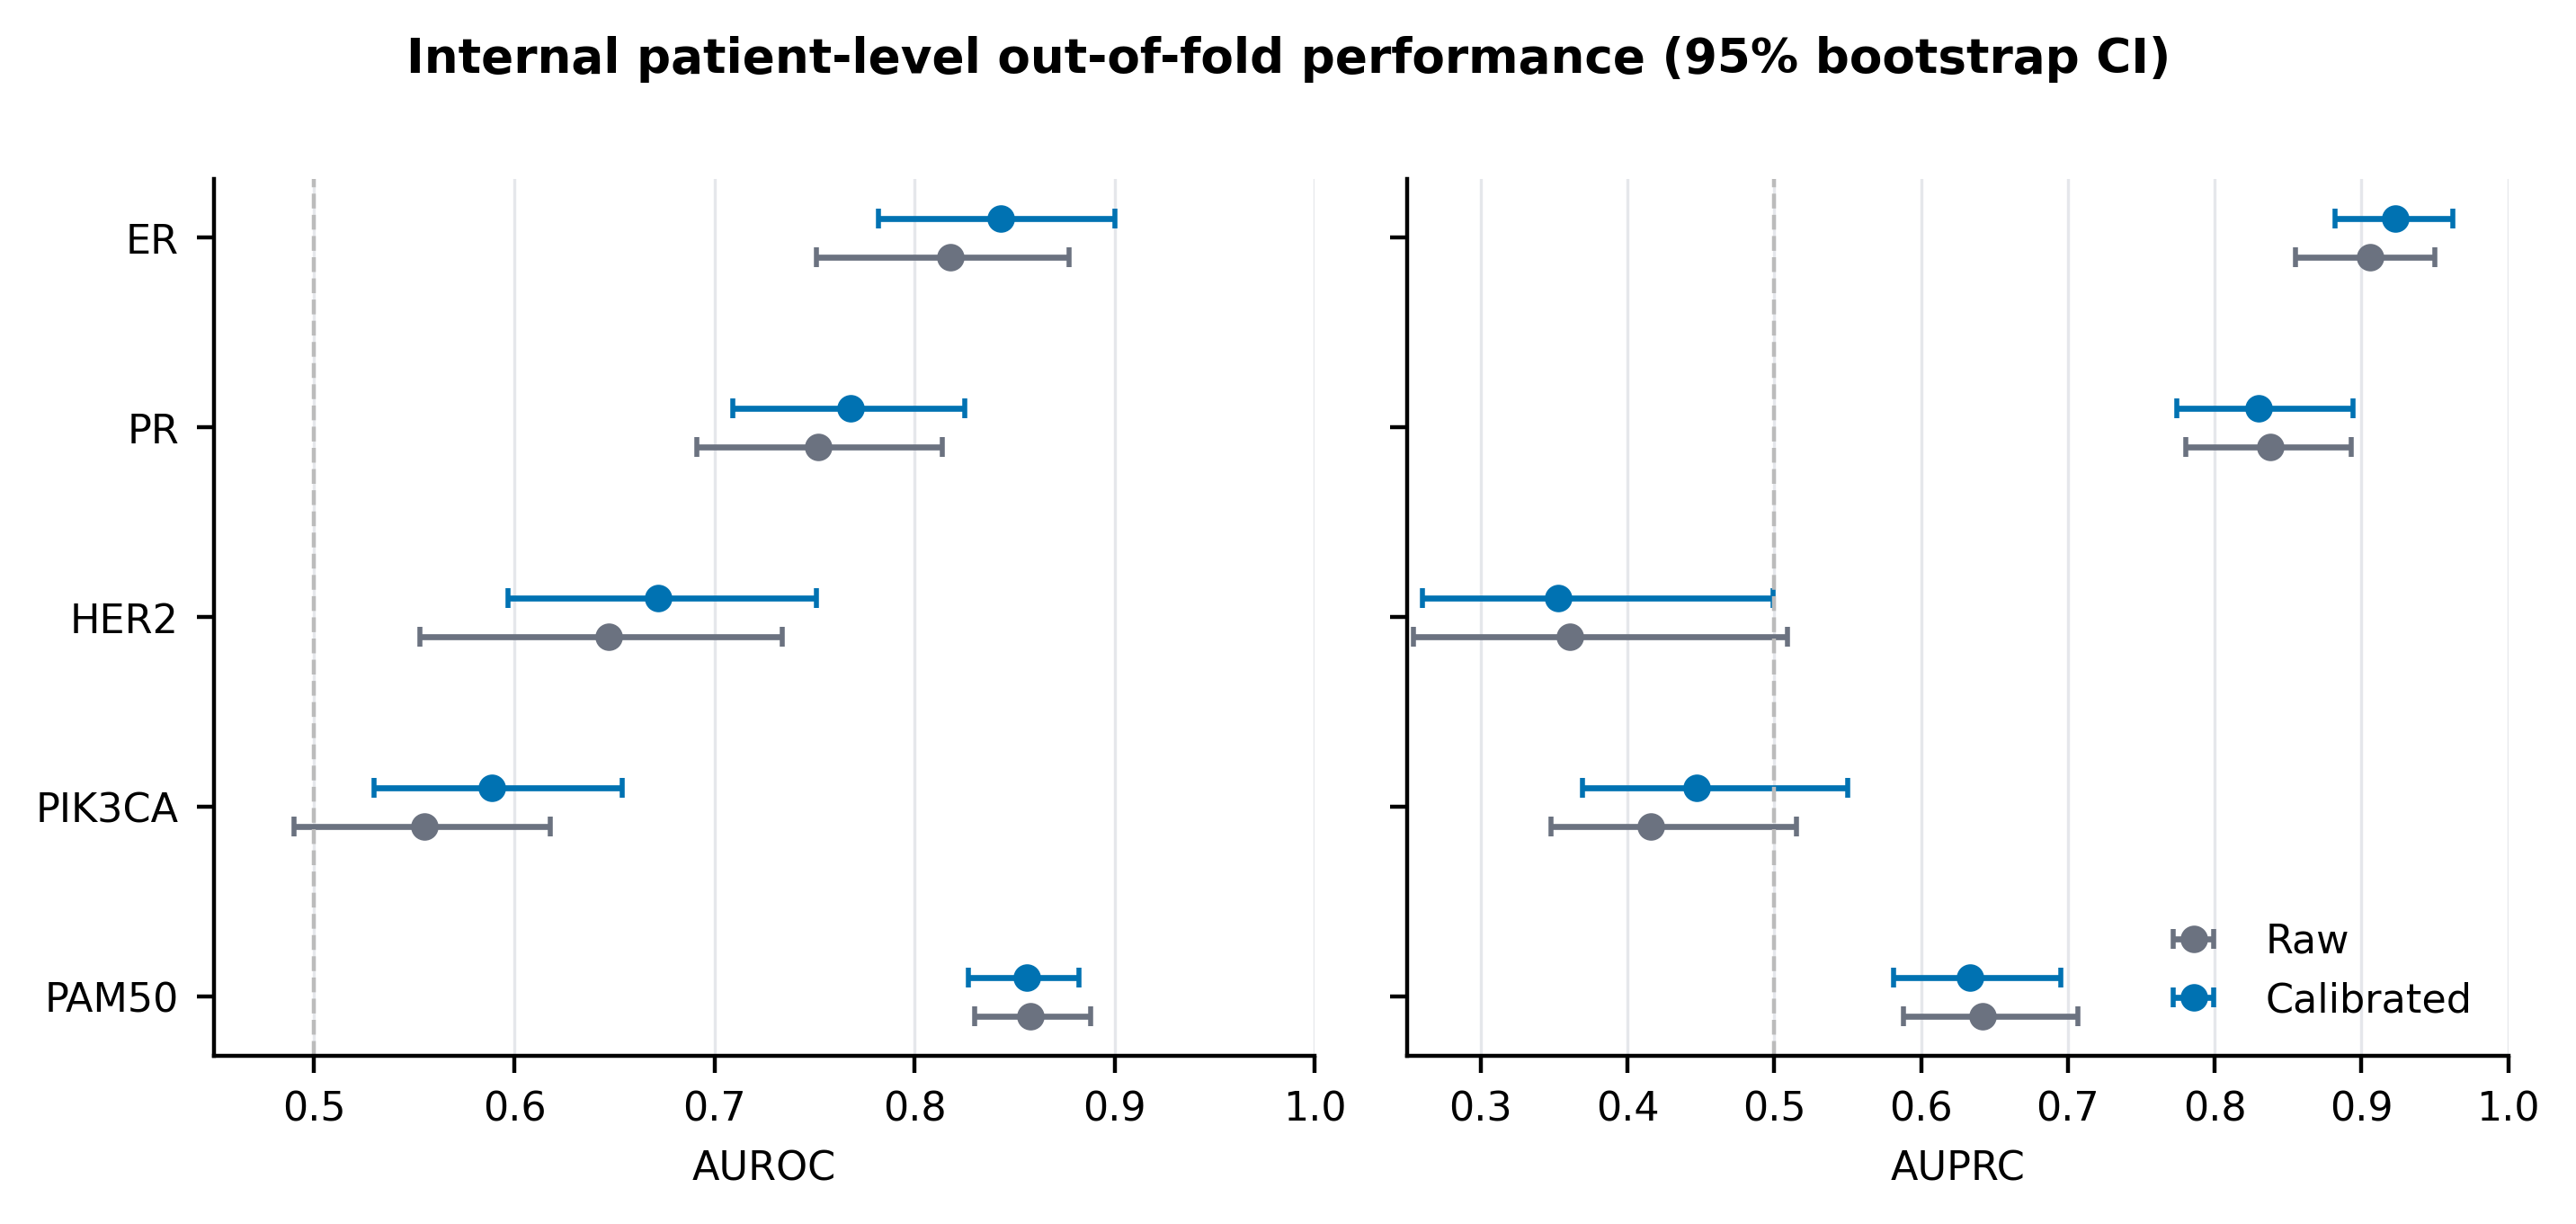
\includegraphics[width=\textwidth]{figures/Figure2_internal_performance.png}
\caption{Internal patient-level discrimination. Pooled out-of-fold AUROC and AUPRC for raw and sigmoid-calibrated predictions, with 95\% confidence intervals from 1,000 patient-level bootstrap replicates. PAM50 metrics are macro-averaged one-versus-rest estimates.}
\label{fig:internal}
\end{figure*}

\subsection{Probability calibration}

Calibration reduced binary probability error more consistently than it altered discrimination (Fig.~\ref{fig:calibration}; Supplementary Tables~S2--S3 and Supplementary Fig.~S2). Brier-score reductions were 0.019 for ER (95\% CI, 0.004--0.035; $p=0.022$), 0.039 for PR (0.018--0.061; $p=0.002$), 0.041 for HER2 (0.020--0.061; $p=0.002$), and 0.089 for \textit{PIK3CA} (0.058--0.120; $p=0.002$). ECE reductions were nominally supported for ER, HER2, and \textit{PIK3CA}, but not PR ($p=0.074$).

Raw binary calibration slopes ranged from 0.039 to 0.257, indicating overly extreme probabilities. Calibrated slopes ranged from 0.861 to 1.043, and calibration-in-the-large intercepts approached zero. Reliability diagrams showed corresponding improvements.

PAM50 showed no clear calibration benefit: Brier-score change was $-0.009$ (95\% CI, $-0.037$ to 0.023; $p=0.579$), while ECE increased by 0.051 ($-0.014$ to 0.101; $p=0.120$). Calibrated classwise slopes were 1.399--2.046. Raw probabilities remained the primary PAM50 analysis.

\begin{figure*}[htbp]
\centering
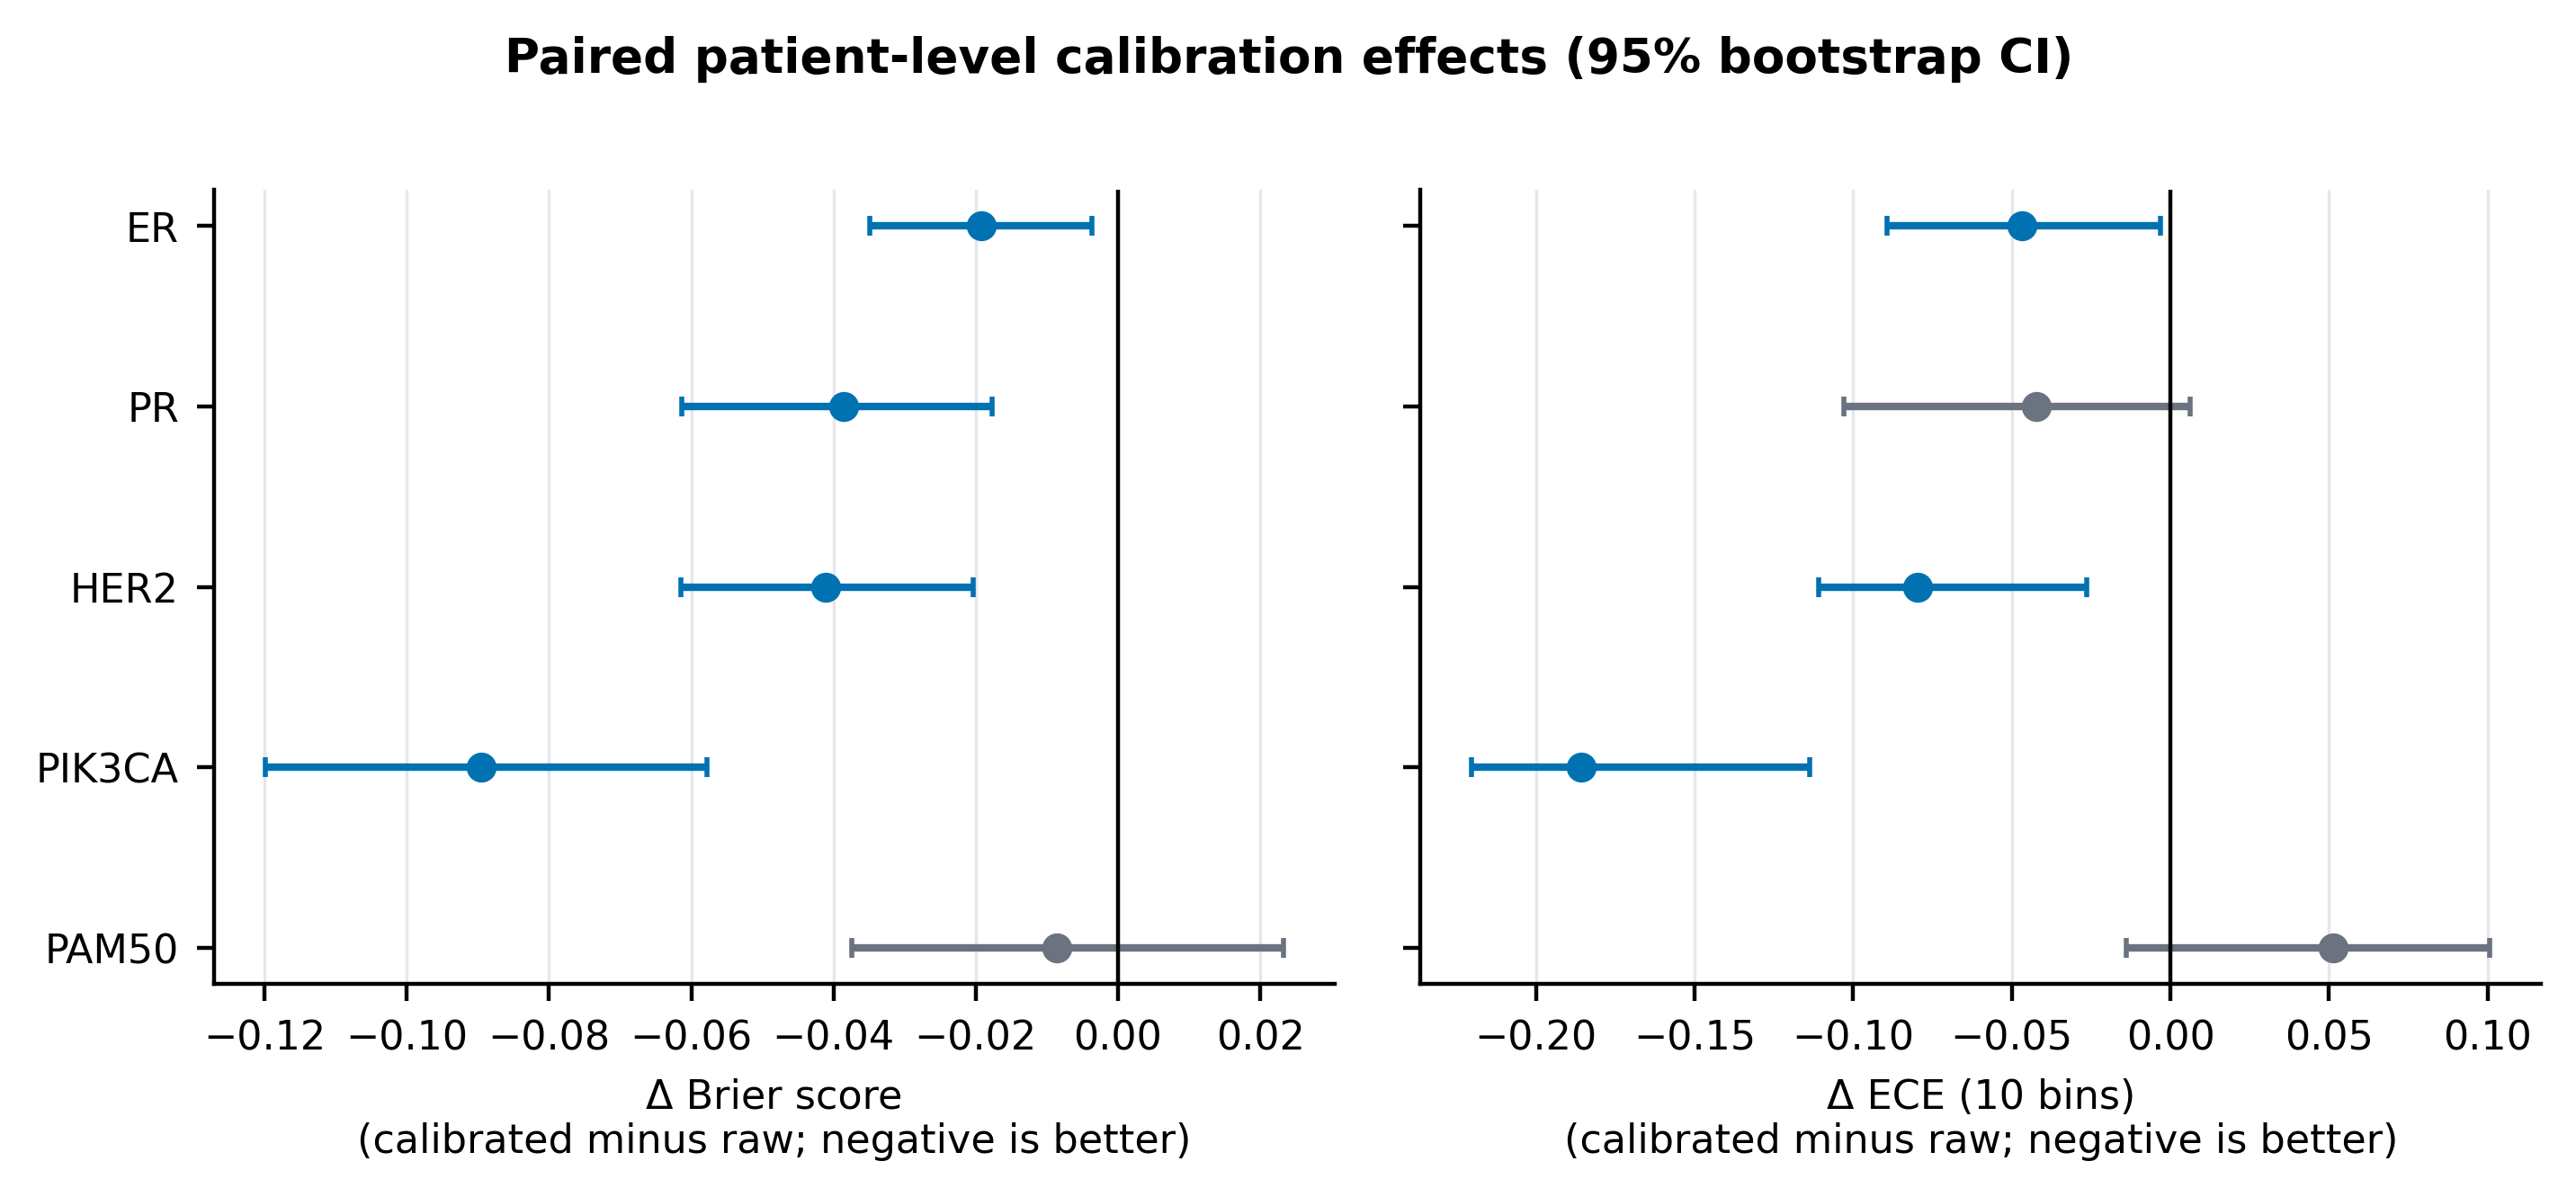
\includegraphics[width=\textwidth]{figures/Figure3_calibration_effects.png}
\caption{Paired calibration effects. Changes in Brier score and ten-bin ECE for calibrated minus raw predictions, with patient-level bootstrap 95\% confidence intervals. Negative values indicate improvement; blue denotes nominal, unadjusted paired-bootstrap $p<0.05$.}
\label{fig:calibration}
\end{figure*}

\subsection{Within-TCGA site-held-out performance}

Site-held-out results varied by endpoint (Table~\ref{tab:sites}; Fig.~\ref{fig:sites}; Supplementary Table~S1). Mean calibrated AUROCs were 0.869 for ER, 0.781 for PR, 0.656 for HER2, and 0.613 for \textit{PIK3CA}; PAM50 mean calibrated macro-AUROC was 0.809.

HER2 had the widest AUROC range (0.577--0.720). At C8, only 32 patients were evaluable; AUROC was 0.577 (95\% CI, 0.345--0.798), and ECE was 0.395 (0.260--0.553). ER and PAM50 retained comparatively strong discrimination, whereas \textit{PIK3CA} remained weak across sites. Small or class-imbalanced test groups produced wide intervals, limiting comparisons between individual TSS codes. These holdouts evaluated within-TCGA transportability, not independent external validity.

\begin{table}[htbp]
\centering
\caption{Calibrated within-TCGA site-held-out performance. Means are unweighted across the four holdout sites; ranges and worst-site values are site-level extrema. PAM50 discrimination metrics are macro-averaged one-versus-rest estimates.}
\label{tab:sites}
\small
\setlength{\tabcolsep}{3pt}
\renewcommand{\arraystretch}{1.15}

\begin{tabularx}{\linewidth}{
@{}l
*{4}{>{\centering\arraybackslash}X}
@{}}
\toprule
\textbf{Endpoint}
& \shortstack{\textbf{Mean}\\\textbf{AUROC}}
& \shortstack{\textbf{AUROC}\\\textbf{range}}
& \shortstack{\textbf{Worst-site}\\\textbf{AUPRC}}
& \shortstack{\textbf{Mean}\\\textbf{ECE}} \\
\midrule
ER              & 0.869 & 0.814--0.931 & 0.833 & 0.093 \\
PR              & 0.781 & 0.730--0.819 & 0.768 & 0.125 \\
HER2            & 0.656 & 0.577--0.720 & 0.297 & 0.199 \\
\textit{PIK3CA} & 0.613 & 0.587--0.661 & 0.404 & 0.101 \\
PAM50           & 0.809 & 0.767--0.827 & 0.568 & 0.123 \\
\bottomrule
\end{tabularx}
\end{table}

\begin{figure*}[htbp]
\centering
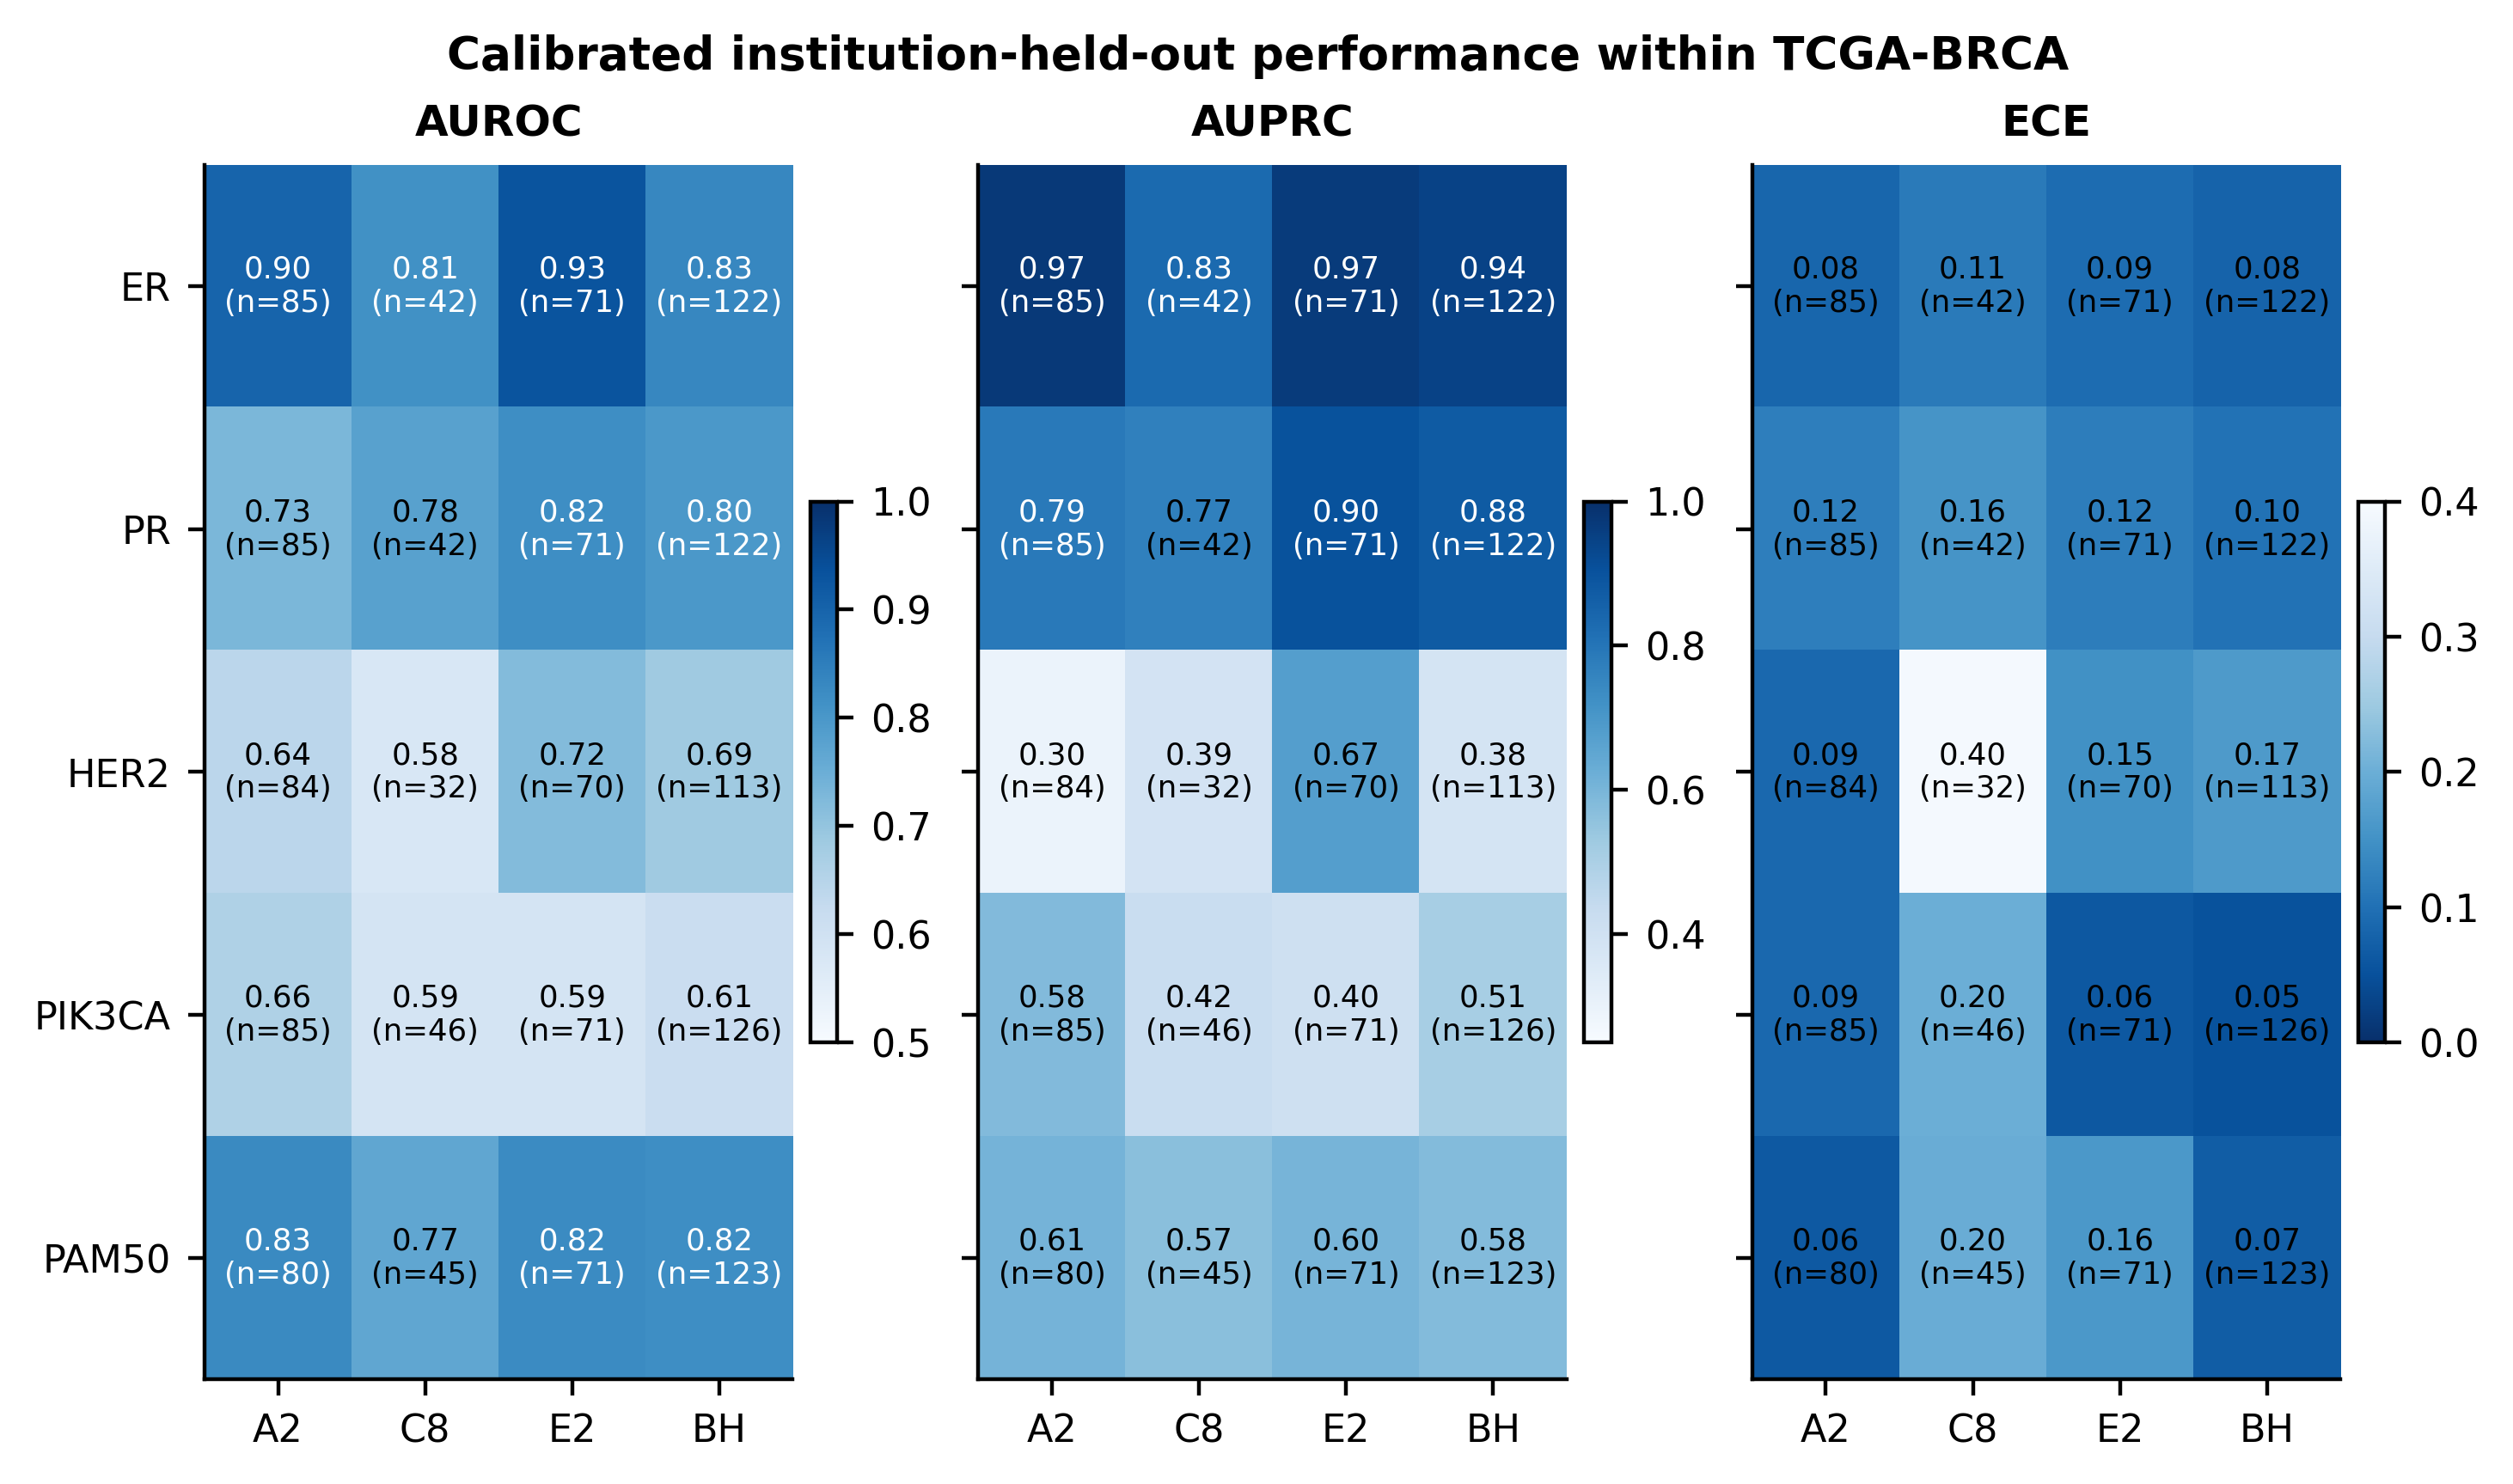
\includegraphics[width=\textwidth]{figures/Figure4_site_holdout.png}
\caption{Within-TCGA site-held-out performance. Calibrated AUROC, AUPRC, and ten-bin top-label ECE for A2, C8, E2, and BH; cells show test-set sizes. Binary endpoints used validation-fitted Platt scaling and PAM50 used temperature scaling. PAM50 discrimination metrics are macro-averaged one-versus-rest estimates.}
\label{fig:sites}
\end{figure*}

\subsection{Representation comparisons}

L2 normalisation increased raw pooled AUROC for ER, PR, HER2, and \textit{PIK3CA}, while PAM50 remained similar (Table~\ref{tab:ablation}; Fig.~\ref{fig:ablation}). Only the \textit{PIK3CA} improvement met the nominal significance threshold: AUROC increased from 0.555 to 0.588 (difference, 0.033; 95\% CI, 0.004--0.064; $p=0.020$; Supplementary Table~S3).

PCA-32 increased \textit{PIK3CA} AUROC to 0.609, but the difference was not nominally supported (0.054; 95\% CI, $-0.009$ to 0.118; $p=0.094$). PAM50 macro-AUROC decreased with PCA-32, PCA-64, and PCA-128 by 0.022 ($p=0.024$), 0.017 ($p=0.004$), and 0.015 ($p=0.002$), respectively. Compression therefore did not uniformly preserve predictive information. All comparisons were exploratory and unadjusted for multiplicity.




\section{Discussion}

Frozen UNI representations captured breast-cancer molecular phenotypes unevenly. ER and four-class PAM50 showed the strongest discrimination, PR was intermediate, and HER2 and \textit{PIK3CA} were weaker. Calibration improved probability accuracy for all binary endpoints but provided no clear benefit for PAM50. Site-held-out evaluation revealed additional endpoint-specific weaknesses, particularly for HER2. Together, these findings show why pooled discrimination alone is insufficient to assess the reliability of histology-based molecular predictions.

The endpoint differences are biologically plausible. ER status and intrinsic subtype reflect broad differentiation programmes that may influence tissue architecture, nuclear features, stromal relationships, and immune composition. Previous studies have linked breast histology to receptor-defined and molecular phenotypes \citep{Couture2018,Rawat2020,Ektefaie2021,Shamai2024}. PAM50 integrates coordinated gene-expression programmes and may therefore have more distributed morphological correlates than a single-gene alteration. Its sensitivity to PCA compression is compatible with predictive information extending beyond the retained components, but does not establish a biological mechanism. Spatial and molecular validation would be needed to test that interpretation.

HER2 and \textit{PIK3CA} highlight the limits of this approach. Morphology may incompletely reflect HER2 protein expression or gene amplification, and the smaller positive group and variable site performance further constrain confidence. \textit{PIK3CA} alterations occur across diverse histological backgrounds, and discrimination remained modest despite the nominal improvement with L2 normalisation. These results provide insufficient evidence for assay substitution. Comparisons with multimodal \textit{PIK3CA} systems require caution because additional clinical inputs and independent multicentre cohorts define a different prediction setting \citep{Miao2026}. Reporting weaker endpoints alongside favourable findings helps establish the boundaries of the representation.

Calibration addressed probability reliability rather than establishing stronger biological signal. Binary Brier scores decreased and calibration slopes approached one under the combined sigmoid-calibration and ensemble procedure. Because this procedure averaged independently fitted models, changes in discrimination cannot be attributed solely to a monotonic probability mapping. For PAM50, classwise slopes above one were consistent with probabilities becoming too compressed; sigmoid calibration was therefore not uniformly beneficial. Calibration methods should be selected and evaluated for each endpoint using development data, with performance assessed on untouched patients \citep{Guo2017,Minderer2021}.

The TSS holdouts also exposed weaknesses that pooled patient splits could obscure. Institutions may differ in phenotype prevalence, staining, processing, scanners, and patient characteristics. Holding out source sites evaluates the combined effect of these differences, but cannot isolate their causes. HER2 performance at C8 illustrates both potential transportability problems and substantial uncertainty: the small test group produced a wide AUROC interval and high ECE. Individual sites should therefore not be ranked from point estimates alone. These experiments address selected TCGA source domains and do not demonstrate generalisation to an unrelated health system.

The frozen encoder and linear probes enabled controlled endpoint comparisons with limited task-specific flexibility. However, hierarchical mean pooling gave equal influence to retained patches within each slide and could dilute tumour-specific signals. Attention-based multiple-instance learning may improve aggregation \citep{Lu2021}, but requires validation of both predictive performance and spatial interpretations. Comparing multiple foundation models would help determine whether the observed limitations are specific to UNI or shared across representations.

Other limitations include retrospective sampling, heterogeneous label sources, small or class-imbalanced endpoint site groups, and the absence of pathologist-annotated tumour regions. The acquisition cohort was a selected subset of TCGA-BRCA rather than a representative sample of the full imaging population. Bootstrap intervals conditioned on completed predictions and did not capture model-retraining variability. Exploratory comparisons were unadjusted for multiplicity. We did not assess prospective workflow impact, treatment decisions, survival benefit, demographic fairness, or cost-effectiveness.

% These findings support further investigation of histology-based molecular prediction as an adjunct for assay prioritisation or quality assurance, rather than evidence of established clinical utility. Future work should combine independent-cohort validation, endpoint-specific calibration, alternative foundation models, and spatially interpretable aggregation. Clinical use would require prospective evidence that image-derived predictions improve testing or care while preserving definitive molecular assessment.



\section{Conclusions and Future Work}
\label{sec:conclusion}

Frozen UNI representations captured breast-cancer molecular phenotypes with endpoint-dependent performance. Discrimination was strongest for ER and four-class PAM50, while HER2 and \textit{PIK3CA} remained less reliably predicted. Calibration improved binary probability accuracy but provided no clear benefit for PAM50. Within-TCGA site holdouts revealed additional variation, supporting joint evaluation of discrimination, calibration, and transportability.

Future work should evaluate independent cohorts, compare foundation models, and investigate spatially interpretable aggregation and endpoint-specific calibration. Prospective studies are needed to establish whether image-derived predictions improve molecular-testing prioritisation or quality assurance. The present findings do not support replacing validated molecular assays.

\section*{Data availability}

Diagnostic WSIs and associated clinical and molecular data are available through the NCI Genomic Data Commons TCGA-BRCA project, subject to applicable access and data-use conditions. PanCancer Atlas molecular annotations are available through cBioPortal. Frozen partitions, patient-level features, derived de-identified metadata, predictions, results, and reproducibility documentation are available in the \href{https://github.com/Gozie01/tcga-brca-cross-site-foundation-model}{GitHub repository} and the \href{https://doi.org/10.5281/zenodo.22668916}{all-version Zenodo record}. Raw WSIs are not redistributed. Patch-level representations are excluded owing to storage requirements but can be regenerated using the released manifests and extraction pipeline.

\section*{Code availability}

The complete analysis and figure-generation code is available through the \href{https://github.com/Gozie01/tcga-brca-cross-site-foundation-model}{GitHub repository} and its \href{https://doi.org/10.5281/zenodo.22668916}{Zenodo record}. Pretrained UNI weights are available from \href{https://huggingface.co/MahmoodLab/UNI}{MahmoodLab/UNI}, subject to its licence and access conditions.

\section*{CRediT authorship contribution statement}

\textbf{C.A.N.:} Conceptualization, Methodology, Software, Data curation, Investigation, Formal analysis, Visualization, Writing -- original draft.
\textbf{S.O.A.:} Methodology, Validation, Writing -- review and editing.
\textbf{G.E.O.:} Methodology, Writing -- review and editing.
\textbf{J.M.L.:} Conceptualization, Methodology, Writing -- review and editing.
\textbf{D.-S.K.:} Conceptualization, Methodology, Supervision, Project administration, Funding acquisition, Resources, Writing -- review and editing.
All authors reviewed and approved the final manuscript.

\section*{Declaration of competing interest}

The authors declare no competing interests.

\section*{Ethics approval and consent to participate}

This study analysed de-identified TCGA-BRCA data from established research repositories. No participants were recruited or contacted, no intervention was performed, and no directly identifiable information was accessed. Under the authors' institutional policies, additional ethics approval and informed consent were not required. Original TCGA data collection followed the relevant ethical approvals and informed-consent procedures.


\section*{Acknowledgements}

This work was supported in part by the Innovative Human Resource Development for Local Intellectualization programme through the Institute of Information \& Communications Technology Planning \& Evaluation (IITP), funded by the Ministry of Science and ICT (MSIT), Republic of Korea (IITP-2026-RS-2020-II201612; 20\%); the Priority Research Centers Program through the National Research Foundation of Korea (NRF), funded by the Ministry of Education, Science and Technology (2018R1A6A1A03024003; 20\%); the Information Technology Research Center support programme through IITP, funded by MSIT (IITP-2026-RS-2024-00438430; 20\%); the Basic Science Research Program through the NRF, funded by the Ministry of Education (RS-2025-25431637; 20\%); and the Regional Innovation System \& Education Regional Growth Innovation LAB programme through the Gyeongbuk RISE Center, funded by the Ministry of Education and Gyeongsangbuk-do, Republic of Korea (2026-RISE-15-105; 20\%).

The funders had no role in the study design, data acquisition, analysis, interpretation, manuscript preparation, or the decision to submit the work.


\section*{Declaration of generative AI and AI-assisted technologies in the writing process}

During manuscript preparation, the authors used OpenAI's ChatGPT to improve language, clarity, and concision. The authors reviewed and edited the assisted content and take full responsibility for the publication.

















% To print the credit authorship contribution details
% \printcredits





\FloatBarrier

% \bibliographystyle{elsarticle-num}
% \bibliography{references}
%% Loading bibliography style file
%\bibliographystyle{model1-num-names}
\bibliographystyle{cas-model2-names}

% Loading bibliography database
\bibliography{cas-refs}

% Biography
%\bio{}
% Here goes the biography details.
%\endbio

%\bio{pic1}
% Here goes the biography details.
%\endbio

\end{document}

